% ============================================================================
%  SABR Volatility Curves, BAW Option Pricing and Historical-Simulation VaR
%  with Full Revaluation
%
%  Build:  tectonic -X compile paper.tex
%  Figures: paper/figures/*.pdf, produced by paper/make_figures.py
% ============================================================================
\documentclass[11pt]{article}

\usepackage[letterpaper,margin=1.15in]{geometry}   % \textwidth = 6.2in exactly,
                                                   % which is what the figures are
                                                   % sized to. Do not change one
                                                   % without the other.
\usepackage{stix2}
\usepackage{amsmath}
\usepackage{booktabs}
\usepackage{graphicx}
\usepackage{caption}
\usepackage{microtype}
\usepackage{array}
\usepackage{longtable}
\usepackage[round,authoryear]{natbib}
\usepackage[hidelinks]{hyperref}

\graphicspath{{figures/}}

% Float placement. Without this the eight full-width figures accumulate and get
% flushed after the bibliography. placeins keeps every float inside its own section.
\usepackage[section]{placeins}
\renewcommand{\topfraction}{0.92}
\renewcommand{\bottomfraction}{0.85}
\renewcommand{\textfraction}{0.06}
\renewcommand{\floatpagefraction}{0.72}
\setcounter{topnumber}{3}
\setcounter{bottomnumber}{2}
\setcounter{totalnumber}{5}

\captionsetup{font=small,labelfont=bf,justification=justified,
              singlelinecheck=false,width=\textwidth}
\captionsetup[table]{skip=4pt}
\captionsetup[figure]{skip=6pt}

\setlength{\parskip}{0pt}
\setlength{\emergencystretch}{2em}

\newcommand{\vp}{\,\text{vol pts}}
\newcommand{\pct}{\,\%}

\title{\bfseries SABR Volatility Curves, BAW Option Pricing and\\
       Historical-Simulation VaR with Full Revaluation\\[4pt]
       \large An implementation and evaluation of the SR-FICC-2013-02\\
       margining methodology on SPY options, with cross-vendor validation\\
       and a two-regime comparison}

\author{[Author name]}
\date{September 2026}

\begin{document}
\maketitle

% ============================================================ ABSTRACT
\begin{abstract}
\noindent
We implement and evaluate the options margining methodology described in a 2013 Fixed
Income
Clearing Corporation rule filing with the U.S.\ Securities and Exchange Commission
(Release No.~34-69470, File No.~SR-FICC-2013-02), which specifies three interlocking
components: a SABR stochastic-volatility curve for the implied volatility smile, the
Barone-Adesi and Whaley (1987) quadratic approximation for American option prices, and
a $99\%$ historical-simulation Value-at-Risk in which every scenario is
\emph{fully revalued} rather than approximated by a delta/gamma expansion. The filing
governs options on interest rate futures; we apply the same machinery to SPY equity
index options, which forces the general cost-of-carry form of the pricer that the
filing's futures options ($b=0$) never exercise. The methodology is run end to end on
two independent reference cases drawn from two independently sourced datasets:
2023-12-29 (OptionsDX end-of-day chains) and 2026-06-01 (Databento OPRA quotes,
353~sessions, acquired for \$8.11). The two cases give $99\%$ one-day VaR of
\$2.4488 and \$4.1216, or $36.89\%$ and $28.58\%$ of position value.
To establish that this difference is a property of the market rather than of the data
feed, we price the \emph{original} reference date from the second vendor using the
unmodified pipeline: the median mid-price difference across 151 common strikes is
\$0.0000 and the median re-implied volatility difference is $0.0000\vp$, with the
put-call-parity forward agreeing to $0.89$ basis points. That check also resolves a
diagnostic left open by the implementation, showing that a wrong-signed kink of
$+0.291\vp$ at the put/call crossover was a vendor artefact while a residual
inconsistency of roughly $+0.15\vp$ beneath it is a genuine market feature reproduced
by both sources to $0.0007\vp$. We quantify two precision floors that the
methodology cannot escape: the quadratic approximation contributes an error of
approximately $1\%$ to every scenario P\&L, amplified $5.5\times$ relative to the
price-level error because its sign changes with moneyness; and the filing's phrase
``linear interpolation'' does not determine a quantile rank convention, an ambiguity
worth $1.46\%$ of VaR in the first case but $21.26\%$ in the second. The dominant
sensitivity in both cases is neither of these but the composition of the lookback
window, which we demonstrate within a single continuous dataset by watching the
April~2025 selloff age out of the window between March and June~2026.
\end{abstract}

% ============================================================ 1. INTRODUCTION
\section{Introduction}

In April 2013 the Fixed Income Clearing Corporation filed a proposed rule change with
the Securities and Exchange Commission seeking to admit options on short-dated interest
rate futures into the one-pot cross-margining program it operated jointly with New York
Portfolio Clearing \citep{ficc2013}. Admitting options to a margining program that had
previously handled only linear instruments required the filing to say how those options
would be valued and how their risk would be measured. The answer it gives rests on three
components, and the interest of the specification lies in how tightly they are coupled.

A SABR curve \citep{hagan2002} supplies an implied volatility at any strike, which is
what makes it possible to price a contract whose own quote is stale or absent. The
Barone-Adesi and Whaley \citeyearpar{baw1987} quadratic approximation converts that
volatility into an American option price, which is required because the contracts carry
an early-exercise right that a European formula prices at zero. Historical simulation
generates roughly a year of alternative next-day market states by replaying observed
daily moves. The binding constraint --- and the reason the first two components are
needed at all --- is that each of those states is \emph{fully revalued}: a fresh
volatility from the curve and a fresh price from the pricer, never a Taylor expansion
in the Greeks. A margining methodology that permitted the expansion would need neither a
smile model nor an American pricer inside its scenario loop, since delta and gamma
computed once at the reference state would suffice.

\subsection{Why SPY rather than interest rate futures options}

We apply the methodology to options on SPDR S\&P 500 ETF Trust (SPY) shares rather
than to the filing's interest rate futures options. Three reasons, in decreasing order
of importance.

First, data. Options on two-year Treasury futures are not available to us at the
strike-by-strike, day-by-day granularity that a smile calibration and a 250-day
historical simulation both require; SPY chains are, from more than one vendor, which is
what makes the cross-vendor validation in Section~\ref{sec:crossvendor} possible at all.
Second, the substitution \emph{exercises more of the methodology, not less}. Options on
futures carry a cost of carry $b=0$, so the pricer collapses to the Black
\citeyearpar{black1976} form and the American premium on a call is structurally
different. SPY is a dividend-paying equity ETF with $b=r-q$, so the general
cost-of-carry pricer must be implemented and $b$ must be obtained from somewhere. We
derive it from the quotes rather than assume it, and one of the two reference cases
turns out to sit on each side of the $b=r$ boundary that determines whether an American
call has any early-exercise value at all. Third, SPY options are American-style, as the
filing's are, so the choice of pricer is not a matter of convenience.

What is lost is that SPY is not the filing's underlying and its smile is not the
filing's smile. This is an evaluation of a \emph{method}, and no claim is made that the
numbers here would be the numbers a clearing house computes.

\subsection{Contributions}

Beyond implementing the specified methodology, this paper contributes three things.

\textbf{An independent-vendor validation of the reference market state.} Every result
in a study of this kind rests on a single day's quotes from a single vendor, and that
dependence is usually acknowledged and then left alone. We instead purchased the same
reference date from a second, structurally different source --- consolidated OPRA
quotes rather than an end-of-day vendor file --- and ran the project's own unmodified
parity and inversion code against it. Section~\ref{sec:crossvendor} reports what agreed,
what did not, and, importantly, one diagnostic of ours that the second source showed to
be unreliable.

\textbf{A second complete reference case, in a different regime and from a different
source.} The same code, with only a configuration file and a data directory changed,
is run on a 2026 reference date built from a dataset we assembled ourselves. Because
the cross-vendor check bounds the feed's contribution, the differences between the two
answers can be attributed to the market with a quantitative bound rather than an
assertion.

\textbf{A within-dataset demonstration of lookback-window aging.} The standard criticism
of unweighted historical simulation --- that a crisis counts fully until the day it
leaves the window and not at all thereafter --- is usually illustrated by comparing
different eras. We show it happening inside one continuous seventeen-month dataset, as
the April~2025 selloff falls off the back of a rolling 250-day window.

We also report several negative and null results plainly, because they bound what this
evaluation establishes: a residual put/call volatility inconsistency that
re-implying the volatilities reduced but did not remove; a diagnostic metric of our own
that a second data source falsified; and the fact that the second reference case, unlike
the first, has no independent price benchmark of its own.

% ============================================================ 2. METHODOLOGY
\section{Methodology}
\label{sec:method}

Throughout, $S$ is the spot price of the underlying, $K$ a strike, $T$ the time to
expiry in years on an ACT/365 basis, $r$ the continuously compounded risk-free rate,
$q$ a continuous dividend yield, $b=r-q$ the cost of carry, and $F=Se^{bT}$ the forward.
Volatilities are quoted in decimal form but differences between them are reported in
\emph{volatility points}, one point being $0.01$ in decimal terms.

\subsection{The market state: forward, carry and the out-of-the-money smile}
\label{sec:forward}

The smile model is written in terms of the forward, so the forward must be established
before anything is calibrated. Rather than assume a dividend yield, we pin $r$
externally to the three-month Treasury constant-maturity yield \citep{fred} and imply
the forward
from put-call parity across liquid near-the-money strikes,
\begin{equation}
  F \;=\; K + e^{rT}\bigl[C(K)-P(K)\bigr],
  \label{eq:parity}
\end{equation}
averaging the per-strike estimates, and then recovering the carry and the implied
dividend yield by inversion,
\begin{equation}
  b=\frac{1}{T}\ln\!\frac{F}{S},
  \qquad
  q=r-b .
  \label{eq:carry}
\end{equation}
The dispersion of the per-strike estimates entering \eqref{eq:parity} is the diagnostic
that the procedure worked, and is reported for both cases in Section~\ref{sec:results}.

Equation~\eqref{eq:parity} holds exactly only for European options, and SPY options are
American, so the put's early-exercise premium biases $F$ slightly low. We quantify that
bias rather than ignore it (Section~\ref{sec:crossover}).

The smile itself is built from out-of-the-money quotes only, split at the forward rather
than at spot: below $F$ the put is taken, above $F$ the call. The in-the-money leg is
illiquid and its quoted volatility unreliable --- at one strike in the 2023 chain the
deep in-the-money call implies $27.2\%$ against $23.2\%$ for the liquid out-of-the-money
put at the same strike --- and including it would give the fit two mutually inconsistent
observations per strike.

\subsection{SABR}

Under SABR \citep{hagan2002} the forward and its volatility follow
\begin{equation}
  \mathrm{d}F_t = \alpha_t F_t^{\beta}\,\mathrm{d}W^{1}_t,
  \qquad
  \mathrm{d}\alpha_t = \nu\,\alpha_t\,\mathrm{d}W^{2}_t,
  \qquad
  \mathrm{d}W^{1}_t\,\mathrm{d}W^{2}_t = \rho\,\mathrm{d}t ,
  \label{eq:sabr-sde}
\end{equation}
with $\alpha_0=\alpha>0$ the volatility level, $\beta\in[0,1]$ the elasticity, $\rho$
the spot/volatility correlation and $\nu\ge 0$ the volatility of volatility. The model
is used through Hagan et al.'s singular perturbation expansion for the Black implied
volatility, which for $K\neq F$ reads
\begin{equation}
  \sigma_{B}(K,F)\;=\;
  \frac{\alpha}{(FK)^{(1-\beta)/2}\,
        \Bigl[1+\frac{(1-\beta)^2}{24}\ln^{2}\!\frac{F}{K}
               +\frac{(1-\beta)^4}{1920}\ln^{4}\!\frac{F}{K}\Bigr]}
  \cdot \frac{z}{x(z)} \cdot \bigl[1+\Theta\,T\bigr],
  \label{eq:hagan}
\end{equation}
where
\begin{equation}
  z=\frac{\nu}{\alpha}(FK)^{(1-\beta)/2}\ln\!\frac{F}{K},
  \qquad
  x(z)=\ln\!\left[\frac{\sqrt{1-2\rho z+z^{2}}+z-\rho}{1-\rho}\right],
  \label{eq:zx}
\end{equation}
\begin{equation}
  \Theta=\frac{(1-\beta)^{2}\alpha^{2}}{24\,(FK)^{1-\beta}}
        +\frac{\rho\beta\nu\alpha}{4\,(FK)^{(1-\beta)/2}}
        +\frac{(2-3\rho^{2})\nu^{2}}{24}.
  \label{eq:theta}
\end{equation}
The factor $z/x(z)$ in \eqref{eq:hagan} is $0/0$ at the money. We do not regularise it
numerically; we branch explicitly on $|\ln(F/K)|$ below a tolerance to the closed-form
limit $z/x(z)\to 1$, giving
\begin{equation}
  \sigma_{B}(F,F)=\frac{\alpha}{F^{1-\beta}}
  \left[1+\left(\frac{(1-\beta)^{2}\alpha^{2}}{24F^{2-2\beta}}
        +\frac{\rho\beta\nu\alpha}{4F^{1-\beta}}
        +\frac{(2-3\rho^{2})\nu^{2}}{24}\right)T\right].
  \label{eq:atm}
\end{equation}
The branch was verified continuous: probing either side of the tolerance and subtracting
the genuine slope contribution implied by the model's own skew leaves an unexplained
excess of $4.5\times10^{-8}$ volatility points, which is floating-point noise.

\paragraph{Calibration.} With $\beta$ fixed, the remaining three parameters are fitted
by unweighted least squares to the observed out-of-the-money volatilities
$\hat{\sigma}_i$ over a restricted set of strikes,
\begin{equation}
  (\hat{\alpha},\hat{\rho},\hat{\nu})
  =\arg\min_{\alpha,\rho,\nu}
   \sum_{i\in\mathcal{M}}\bigl[\sigma_{B}(K_i,F;\alpha,\beta,\rho,\nu,T)-\hat{\sigma}_i\bigr]^{2},
  \qquad
  \mathcal{M}=\Bigl\{i:\bigl|\tfrac{K_i}{F}-1\bigr|\le 0.15\Bigr\}.
  \label{eq:objective}
\end{equation}
The optimisation is run from twelve starting points with bounds that scale correctly
with $\beta$; the upper bound on $\alpha$ is $5F^{1-\beta}$, since at $\beta=1$ the
parameter is a proportional volatility of order $0.1$ while at $\beta=0$ the model is
normal and $\alpha$ is an absolute volatility in dollars of order $50$.

\paragraph{Why $\beta$ is fixed and not fitted.} The filing specifies SABR but states no
value for $\beta$. We fix $\beta=1$. The reason is not convention but identification:
$\beta$ and $\rho$ both control the skew and trade off against one another almost
exactly, so a joint fit wanders along a flat valley of the objective. Table~\ref{tab:ident}
makes this quantitative --- across the full range $\beta\in[0,1]$ the root-mean-square
fit error moves by $0.04\vp$, which is nothing, while $\hat{\alpha}$ swings by a factor
of $476$ and $\hat{\rho}$ slides to compensate. Fitting both would produce parameters
that jump from day to day while the fit quality never improves. Setting $\beta=1$ makes
the model lognormal, matching the convention in which equity index volatilities are
quoted, and leaves $\rho$ as the sole skew parameter.

A second consideration is cross-asset, and it runs the other way. A native fixed-income
application of this methodology would point towards \emph{Normal} SABR, $\beta=0$: on
options on interest rate futures the forward can sit near zero or turn negative, where
lognormal dynamics are undefined, and the additive dynamics of \eqref{eq:sabr-sde} at
$\beta=0$ remain well posed and match the convention in which rate volatility is quoted.
Fixing $\beta=1$ here follows from the move to an equity index underlying, whose forward
is strictly positive and whose volatilities are quoted lognormally. The elasticity is
thus the one structural parameter that the change of asset class genuinely determines;
carrying the remaining components across unchanged is itself a test of how far the
specification generalises beyond the instrument it was written for.

\paragraph{Why the calibration band is restricted.} Equation~\eqref{eq:hagan} is an
asymptotic expansion whose accuracy degrades away from the money, and the far wings of an
SPY chain are penny quotes: in the 2023 chain, $35$ of the $151$ out-of-the-money strikes
have a mid below \$0.10 with a median relative spread of $40\%$. In an unweighted
objective such as \eqref{eq:objective} those quotes carry the same weight as
at-the-money quotes with a one-cent spread, and they would drag the fit away from the
region that matters. Restricting $\mathcal{M}$ to $|K/F-1|\le0.15$ addresses both
problems at once; Table~\ref{tab:ident} reports the sensitivity to that choice.

\subsection{Barone-Adesi and Whaley}

The generalised Black-Scholes-Merton price with cost of carry \citep{black1973,merton1973}
is
\begin{equation}
  c(S,K,T)=Se^{(b-r)T}N(d_1)-Ke^{-rT}N(d_2),
  \qquad
  d_{1}=\frac{\ln(S/K)+(b+\tfrac{1}{2}\sigma^{2})T}{\sigma\sqrt{T}},
  \quad d_2=d_1-\sigma\sqrt{T},
  \label{eq:gbsm}
\end{equation}
which reduces to Black's futures-option formula at $b=0$ and to Black-Scholes at $b=r$.
Barone-Adesi and Whaley \citeyearpar{baw1987} approximate the American price as the
European price plus a premium of closed form. Writing
\begin{equation}
  M=\frac{2r}{\sigma^{2}},\qquad
  \mathcal{N}=\frac{2b}{\sigma^{2}},\qquad
  k=1-e^{-rT},\qquad
  q_{1,2}=\frac{-(\mathcal{N}-1)\mp\sqrt{(\mathcal{N}-1)^{2}+4M/k}}{2},
  \label{eq:baw-roots}
\end{equation}
the American call and put are
\begin{equation}
  C(S,K,T)=
  \begin{cases}
    c(S,K,T)+A_2\left(\dfrac{S}{S^{*}}\right)^{q_2}, & S<S^{*},\\[10pt]
    S-K, & S\ge S^{*},
  \end{cases}
  \qquad
  A_2=\frac{S^{*}}{q_2}\Bigl[1-e^{(b-r)T}N\bigl(d_1(S^{*})\bigr)\Bigr],
  \label{eq:baw-call}
\end{equation}
\begin{equation}
  P(S,K,T)=
  \begin{cases}
    p(S,K,T)+A_1\left(\dfrac{S}{S^{**}}\right)^{q_1}, & S>S^{**},\\[10pt]
    K-S, & S\le S^{**},
  \end{cases}
  \qquad
  A_1=-\frac{S^{**}}{q_1}\Bigl[1-e^{(b-r)T}N\bigl(-d_1(S^{**})\bigr)\Bigr],
  \label{eq:baw-put}
\end{equation}
where the critical prices $S^{*}$ and $S^{**}$ --- the exercise boundaries --- solve the
value-matching conditions
\begin{align}
  S^{*}-K   &= c(S^{*},K,T)   + \Bigl[1-e^{(b-r)T}N\bigl( d_1(S^{*})  \bigr)\Bigr]\frac{S^{*}}{q_2},
  \nonumber\\
  K-S^{**}  &= p(S^{**},K,T)  - \Bigl[1-e^{(b-r)T}N\bigl(-d_1(S^{**}) \bigr)\Bigr]\frac{S^{**}}{q_1}.
  \label{eq:critical}
\end{align}
We solve \eqref{eq:critical} by Newton-Raphson from the standard seed, with each iterate
clamped into the region where a boundary can economically lie ($S^{*}>K$ for a call,
$S^{**}\in(0,K)$ for a put) and with an explicit error raised for a call when $b\ge r$,
where no finite boundary exists.

A European price will not serve here. When $b<r$ the American call carries a genuine
early-exercise premium, and the American put carries one in every regime; on the 2023
reference contract that premium is \$0.29 on a \$6.47 price, or $4.7\%$ of the option's
value, which is not a rounding error in a margin calculation. The approximation itself
is not exact, and Section~\ref{sec:baw-results} measures what it costs.

\subsection{Historical simulation with full revaluation}

Let $S_0$ be the reference spot and $\{S_{-N},\dots,S_{0}\}$ the closing price series over
the lookback. Simple daily returns
\begin{equation}
  r_i=\frac{S_{-N+i}}{S_{-N+i-1}}-1,\qquad i=1,\dots,N,
  \label{eq:returns}
\end{equation}
are applied to the reference spot to generate $N=250$ alternative next-day states. For
each,
\begin{equation}
  \tilde{S}_i = S_0(1+r_i),
  \qquad
  \tilde{F}_i = \tilde{S}_i e^{bT},
  \qquad
  \tilde{\sigma}_i = \sigma_{B}\bigl(K,\tilde{F}_i;\hat{\alpha},\beta,\hat{\rho},\hat{\nu},T\bigr),
  \qquad
  \tilde{V}_i = V^{\mathrm{BAW}}\bigl(\tilde{S}_i,K,T,r,b,\tilde{\sigma}_i\bigr),
  \label{eq:reval}
\end{equation}
and the scenario profit and loss for a long position of one contract is
$L_i=\tilde{V}_i-V_0$, where $V_0$ is the reference price computed the same way.

Three properties of \eqref{eq:reval} are decisions rather than mechanics. The calibrated
parameters are held fixed and the curve is re-evaluated at the \emph{new} forward, so
the smile is pinned to moneyness rather than to strike. Time to expiry is held fixed at
its reference value, excluding theta, which would otherwise shift every scenario down by
approximately the same amount and inflate the VaR irrespective of market direction. And
the volatility surface is not itself shocked: $\tilde{\sigma}_i$ moves only because
$\tilde{F}_i$ moves. The consequences of all three are quantified in
Section~\ref{sec:limitations}.

The step the filing forbids is the Taylor alternative,
\begin{equation}
  L_i^{\Delta}=\Delta\,(\tilde{S}_i-S_0),
  \qquad
  L_i^{\Delta\Gamma}=\Delta\,(\tilde{S}_i-S_0)+\tfrac{1}{2}\Gamma\,(\tilde{S}_i-S_0)^{2}.
  \label{eq:taylor}
\end{equation}
We compute \eqref{eq:taylor} deliberately, as a counterfactual only, to measure in
dollars what the prohibition buys; it is never used for a reported risk number.

\subsection{Value-at-Risk by interpolation between order statistics}
\label{sec:var-method}

Let $L_{(1)}\le L_{(2)}\le\cdots\le L_{(N)}$ be the ordered scenario P\&Ls and let
$p=1-c=0.01$ be the tail probability at confidence $c=99\%$. The filing specifies linear
interpolation to the threshold. Writing the fractional rank as
\begin{equation}
  h=(N-1)\,p,
  \qquad
  k=\lfloor h\rfloor,
  \qquad
  w=h-k,
  \label{eq:rank}
\end{equation}
the interpolated quantile and the reported risk measures are
\begin{equation}
  \hat{Q}=L_{(k+1)}+w\bigl(L_{(k+2)}-L_{(k+1)}\bigr),
  \qquad
  \mathrm{VaR}=-\hat{Q},
  \qquad
  \mathrm{ES}=-\frac{1}{|\mathcal{B}|}\sum_{i\in\mathcal{B}}L_i,
  \quad
  \mathcal{B}=\{i: L_i\le\hat{Q}\}.
  \label{eq:var}
\end{equation}
VaR and expected shortfall are reported throughout as \emph{positive loss magnitudes};
the quantile retains its natural sign and is negated once, at the point of reporting. A
position that lost nothing even at its first percentile would produce a negative VaR,
and our implementation flags that case rather than clipping it to zero.

Equation~\eqref{eq:rank} is a choice, and the filing's wording does not make it. The
definition $h=(N-1)p$ is R's type 7 and NumPy's default; $h=Np$ and $h=(N+1)p-1$ (R's
type 6, the Weibull convention) are both in common use \citep{hyndman1996}. We implement
the interpolation arithmetically rather than by library call, precisely so that the
convention is a stated assumption rather than an inherited default, and we report the
sensitivity in Section~\ref{sec:rank}. Expected shortfall as defined in \eqref{eq:var}
is the simple mean of the breaching scenarios rather than an integrated tail expectation
\citep{acerbi2002}; at $N=250$ and $p=0.01$ only three scenarios breach, so it is
correspondingly noisy.

\paragraph{Weighting.} The simulation is unweighted: every day in the window counts
equally. This matches the filing and departs from common practice, which would apply
exponential decay \citep{boudoukh1998} or rescale historical returns by the ratio of
current to historical volatility \citep{baroneadesi1999}. The deviation is deliberate,
made to match the specification rather than to improve the estimate, and
Section~\ref{sec:window} shows what it costs.

% ============================================================ 3. DATA
\section{Data}
\label{sec:data}

Two datasets support two reference cases. They differ in vendor, in structure, in the
period they cover and in how much of the preparation we did ourselves, which is the point:
a methodology that transfers between them has been shown to transfer, not asserted to.

\subsection{OptionsDX end-of-day chains, 2010--2023}

The first case uses SPY end-of-day option chains published by OptionsDX \citep{optionsdx}
and widely
mirrored, fourteen annual files covering 2010--2023. Each row is one (quote date, expiry,
strike) triple carrying both the call and the put leg with bid, ask, last, volume and a
vendor-supplied implied volatility. Raw column names are wrapped in square brackets, a
vendor quirk stripped on load.

The underlying price series is taken from the \texttt{UNDERLYING\_LAST} field inside
these same files rather than from a separate equity feed, so that spot remains
synchronous with the option quotes it is paired against. That field is the unadjusted
SPY price, which means SPY's four annual ex-dividend dates appear in the return sample
as spurious down-moves of roughly $0.4\%$. We accept this: the option contracts are
written on the unadjusted price, so shocking the unadjusted price is internally
consistent, and none of the four falls inside the reference lookback window.

\paragraph{A vendor defect, found and bounded.} Validating the price series against a
derived NYSE calendar exposed a date-stamping fault in the 2022 file. Four genuine
trading days are absent (2022-05-11, 06-17, 06-24 and 12-16) and nine rows are stamped
on days the exchange was closed (including 2022-01-17, 07-04 and 11-24). The two faults
damage a return sample in opposite directions. A missing session compresses two days of
movement into one return and manufactures a tail observation that never occurred: the
2022-12-15 to 2022-12-19 interval appears as a single $-2.49\%$ move when it was in fact
$-1.65\%$ followed by $-0.85\%$. A phantom row on a closed market carries a stale price
forward and injects a spurious near-zero return, diluting the tail instead. \emph{Zero
defects fall inside the 250-day window used for the reference case}, which begins
2022-12-30; the check is re-run on every execution rather than assumed.

\subsection{Databento OPRA quotes, 2025--2026}
\label{sec:databento}

The second case uses a dataset we assembled from Databento \citep{databento}: 353 trading
sessions from
2025-01-02 to 2026-06-01, 11{,}036{,}871 quote records reshaped into 1{,}880{,}602 rows,
acquired for \$8.11 in total.

Three schemas were used, each chosen for what it structurally contains. Consolidated
best-bid/offer bars at one-minute resolution (\texttt{cbbo-1m}, \texttt{OPRA.PILLAR})
supply a two-sided quote for every listed strike including the illiquid wings, which is
the whole smile. Trade-derived alternatives were rejected for exactly that reason: an
option that does not trade produces no bar, and the far wings that pin the SABR skew and
curvature trade rarely or never on a given day, so most of the smile would simply be
absent. Instrument definitions (\texttt{definition}, same dataset) supply strike, expiry
and option type for each numeric instrument identifier, without which a quote row cannot
be attached to a strike at all. Daily consolidated bars for SPY itself
(\texttt{ohlcv-1d}, \texttt{EQUS.SUMMARY}) supply \texttt{UNDERLYING\_LAST}, since OPRA
carries no underlying price.

The pull takes a three-minute pre-close window, 15:57--16:00 ET, and keeps each
contract's last bar within it, so that a contract quoted only in an earlier minute keeps
that quote rather than being dropped. The window is resolved per date with a timezone
database rather than a hardcoded UTC offset: 16:00 ET is 20:00 UTC in summer and 21:00
UTC in winter, and getting that wrong silently returns the wrong three minutes.

Three preparation problems are worth recording because each was invisible to a naive
approach and each is a class of defect rather than a one-off.

\textbf{Early closes.} The NYSE closes at 13:00 ET on roughly three days a year. Those
remain trading days, so a derived calendar reports them as ordinary and a 16:00 window
looks entirely normal while sitting three hours after the bell. Three such sessions in
range returned no data at all; pulled at the 13:00 close they returned normal volumes of
26{,}022, 31{,}440 and 26{,}959 rows against a 30{,}273 median. This never surfaced in
the 2010--2023 work because an end-of-day vendor stamps one row per day regardless of
session length.

\textbf{A one-off closure.} 2025-01-09 failed differently, with no symbol resolving at
all: the exchange was closed for a national day of mourning. The session count is
therefore 353, not 354. The two failure modes are distinguishable --- on a short session
the symbols resolve and the window is merely empty --- and the distinction is now
documented in the acquisition code.

\textbf{Definition coverage.} Instrument definitions were first pulled quarterly, on the
reasoning that they are largely static. They are not static enough: contracts listed
between anchor dates have no definition, and the match rate decayed from $100\%$ near an
anchor to $89.3\%$ by 2026-03-17. A per-session definition snapshot for every day in
range took the match rate to $100.0000\%$ across all 11{,}036{,}871 rows, at a cost of
\$6.34 against \$0.12 --- the reference data cost roughly four times the quote data.

One column in the reshaped dataset is not what its name suggests, and the consequence
propagates into Section~\ref{sec:results}. The volatility columns \texttt{C\_IV} and
\texttt{P\_IV} hold European Black-76 volatilities that we computed from the mid on the
parity forward, not a vendor's numbers. They exist because the smile constructor filters
on that column and runs before the re-implying step can replace it, so a null column
returns an empty smile. The inversion round-trips to $3.4\times10^{-13}$ in price. The
consequence is that the before/after comparison of Section~\ref{sec:reimply} measures
something different in each case: in 2023 it measures vendor error \emph{plus} the
European-to-American correction, in 2026 the correction alone. The two are therefore not
comparable baselines, and no inference about relative data quality should be drawn from
the fact that the 2026 correction is the smaller of the two --- it is smaller because it
contains one term rather than two.

\subsection{Cross-vendor validation of the reference market state}
\label{sec:crossvendor}

Before extending anything, we purchased the \emph{original} reference date, 2023-12-29,
from Databento and ran the project's own \texttt{imply\_forward\_from\_parity} and
implied-volatility inversion against it without modification, so that every difference
below is attributable to the data rather than to the method. Cost: \$0.0390.

The join was verified independently before any comparison: the OSI symbol carried on each
quote matches the symbol on its definition for all 312 instruments in the reference
expiry, with zero mismatches, and the joined chain yields 156 strikes with both legs ---
exactly the 156 the OptionsDX chain contains. Table~\ref{tab:crossvendor} reports the
comparison and Figure~\ref{fig:crossvendor} shows it strike by strike.

\begin{table}[t]
\centering
\small
\caption{Cross-vendor comparison of the 2023-12-29 reference state. The project's own
parity and inversion code was run unchanged against Databento OPRA quotes, so every
difference is attributable to the data. Every quantity agrees within ordinary
cross-vendor noise; the two entries that do not sit at zero are examined in the text.}
\label{tab:crossvendor}
\begin{tabular}{lrrr}
\toprule
Quantity & OptionsDX & Databento OPRA & Difference \\
\midrule
Chain strikes, expiry 2024-02-16      & 156 & 156 & 0 \\
Parity forward (\$)                   & 478.8920 & 478.8495 & $-0.0425$ \ (0.89 bp) \\
Forward dispersion (\$)               & 0.203 (22 strikes) & 0.182 (32 strikes) & tighter \\
Implied dividend yield (\%)           & $-0.1926$ & $-0.1265$ & $+0.066$ pp \\
\$475 put, bid / ask (\$)             & 6.51 / 6.54 & 6.58 / 6.61 & mid $+0.0700$ \\
BAW theoretical $-$ market mid (\$)   & $+0.1141$ & $+0.0441$ & closer to theory \\
Crossed out-of-the-money quotes       & 2 ($K=477,478$) & 0 & --- \\
\midrule
\multicolumn{4}{l}{\emph{Across the 151 common out-of-the-money strikes}}\\
Median mid price difference (\$)      & --- & --- & 0.0000 \\
Median re-implied IV difference       & --- & --- & $0.0000\vp$ \\
Mean re-implied IV difference         & --- & --- & $-0.0168\vp$ \\
95th percentile $|$IV difference$|$   & --- & --- & $0.2286\vp$ \\
Strikes differing by more than $1\vp$ & --- & --- & 1 of 151 \\
Re-implied crossover gap, $476\!\to\!479$ & $-0.2088$ & $-0.2164$ & $0.0076\vp$ \\
\bottomrule
\end{tabular}
\end{table}

\begin{figure}[t]
\centering
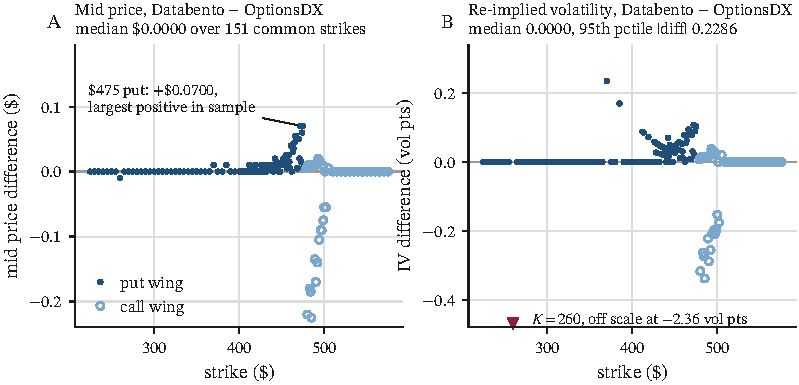
\includegraphics[width=\textwidth]{fig_crossvendor.pdf}
\caption{The 2023-12-29 reference date priced from two independent vendors, strike by
strike. \textbf{A:} mid-price differences sit on zero across the chain; the median over
151 common strikes is exactly \$0.0000. The largest positive difference, $+\$0.0700$,
falls on the \$475 put --- the single contract the headline VaR rests on --- and both
vendors quote a three-cent spread there, so the gap is snapshot timing rather than
disagreement about value. The negative cluster near \$490 is the call wing, where the
two vendors' snapshots diverge by up to $-\$0.225$. \textbf{B:} re-implied volatility
differences, median $0.0000\vp$. Exactly one strike of 151 differs by more than one
volatility point and it is plotted off scale: $K=260$ is a deep-wing penny put quoted
0.01/0.02 against a project mid of 0.025, so a one-cent disagreement is amplified into
$2.36\vp$ by near-zero vega. Rescaling the axis to contain it would hide the finding,
which is that the bulk lies within $\pm0.35\vp$.}
\label{fig:crossvendor}
\end{figure}

\paragraph{What the check establishes.} The OptionsDX-derived reference state is
independently corroborated; the instrument mapping works; and the project's parity and
inversion code runs unchanged against a structurally different source and produces
consistent results. This is what licenses treating any later difference between the two
reference cases as a market difference rather than a feed difference, and
Section~\ref{sec:staged} makes that argument quantitatively.

\paragraph{What it does not establish.} It validates one date. A rebuild of a 2025--2026
period rests on a mapping confirmed on a single day, and no second source has been
purchased for the 2026 reference date itself. Nor are the two objects being compared
identical in kind: a consolidated best-bid/offer at a minute boundary is not the same
thing as an end-of-day vendor snapshot. They agree closely here, but a rule for reducing
minute bars to an end-of-day equivalent is a modelling decision, not a data pull, and it
is ours. Finally, the ``implied spot'' agreement sometimes quoted in such comparisons is
not available here and we do not report one: OPRA carries no underlying price, so spot
cannot be read from these data at all.

% ============================================================ 4. RESULTS
\section{Results}
\label{sec:results}

The methodology of Section~\ref{sec:method} was run end to end twice. The pricing,
calibration, simulation and VaR code is byte for byte identical between the two runs;
only a configuration file and a data directory differ. Table~\ref{tab:config} states
both reference configurations, distinguishing quantities assumed from quantities derived
from the quotes.

\begin{table}[t]
\centering
\small
\caption{The two reference configurations. Only two inputs are assumed --- the risk-free
rate, pinned externally to the same FRED series in both cases, and the SABR elasticity
$\beta$. The forward, the cost of carry and the implied dividend yield are all derived
from the quotes by \eqref{eq:parity} and \eqref{eq:carry}; the SABR parameters are fitted
by \eqref{eq:objective}. The calibration band, the elasticity, the quote filters and the
confidence level are deliberately held identical across the two cases, so that a
comparison of results is not confounded by a comparison of method.}
\label{tab:config}
\begin{tabular}{llll}
\toprule
Quantity & 2023-12-29 & 2026-06-01 & Provenance \\
\midrule
Data source              & OptionsDX EOD      & Databento OPRA      & --- \\
Reference expiry         & 2024-02-16         & 2026-07-17          & standard monthly \\
Days to expiry           & 49                 & 46                  & calendar, ACT/365 \\
$T$ (years)              & 0.13425            & 0.12603             & derived \\
Spot $S$ (\$)            & 475.31             & 758.54              & observed close \\
Risk-free rate $r$ (\%)  & 5.4000             & 3.6600              & \textbf{assumed}, FRED DGS3MO \\
Forward $F$ (\$)         & 478.892            & 760.224             & \textbf{derived}, put-call parity \\
Forward dispersion (\$)  & 0.203 (22 strikes) & ---                 & derived \\
Cost of carry $b$ (\%)   & 5.5926             & 1.7601              & \textbf{derived} \\
Dividend yield $q$ (\%)  & $-0.1926$          & $+1.8999$           & \textbf{derived} \\
Carry regime             & $b>r$              & $b<r$               & consequence \\
\midrule
Chain strikes            & 156                & ---                 & observed \\
Smile strikes (OTM)      & 151 (112 P, 39 C)  & 197 (129 P, 68 C)   & after quality filters \\
Calibration strikes      & 103                & 125                 & $|K/F-1|\le0.15$ \\
SABR $\beta$             & 1.0                & 1.0                 & \textbf{assumed}, not fitted \\
SABR $\hat{\alpha}$      & 0.109797           & 0.136311            & fitted \\
SABR $\hat{\rho}$        & $-0.524225$        & $-0.633712$         & fitted \\
SABR $\hat{\nu}$         & 2.132810           & 2.201313            & fitted \\
Fit RMSE                 & $0.2346\vp$        & $0.2080\vp$         & fitted \\
\midrule
Position                 & $+1\times\$475$ put & $+1\times\$759$ put & --- \\
Moneyness of position    & $0.065\%$ OTM      & $0.061\%$ ITM       & --- \\
SABR volatility at $K$   & $11.7554\%$        & $13.9399\%$         & derived \\
Position value $V_0$ (\$)& 6.639087           & 14.422074           & derived \\
Lookback window          & 2023-01-03 --                   & 2025-06-03 --                   & 250 sessions \\
                         & \quad 2023-12-29               & \quad 2026-06-01               &              \\
Confidence level         & 99\%               & 99\%                & from the filing \\
\bottomrule
\end{tabular}
\end{table}

\subsection{Case 1: 2023-12-29, OptionsDX}
\label{sec:case1}

\subsubsection{Market state and smile construction}

The reference expiry carries 156 strikes from \$210 to \$575, reduced to a 151-strike
out-of-the-money smile after quality filters, with quoted volatilities running from
$9.94\%$ to $64.20\%$. Twenty-two liquid near-the-money strikes enter the parity
calculation \eqref{eq:parity} and agree on the forward to a standard deviation of
\$0.203, roughly four basis points of spot; that tightness is the evidence the procedure
worked.

The forward implies a dividend yield of $-0.1926\%$ --- essentially zero, and correctly
so. SPY's December 2023 ex-dividend date was the 15th and the next fell on 2024-03-15, so
no dividend falls between the reference date and the expiry. Substituting SPY's
approximately $1.4\%$ trailing yield would have mispriced the forward by about \$0.90,
roughly four strike increments, and tilted the entire smile. The near-zero implied yield
is independent corroboration that the $5.40\%$ rate assumption is sound.

\subsubsection{SABR calibration}
\label{sec:case1-sabr}

Fitting \eqref{eq:objective} over the 103 strikes within $15\%$ of the forward gives
$\hat{\alpha}=0.109797$, $\hat{\rho}=-0.524225$, $\hat{\nu}=2.132810$, with a
root-mean-square error of $0.2346\vp$ and a maximum absolute error of $0.5075\vp$. The
correlation parameter is negative, as an equity index requires. Panel~A of
Figure~\ref{fig:sabr} shows the fit and its residuals.

\begin{figure}[t]
\centering
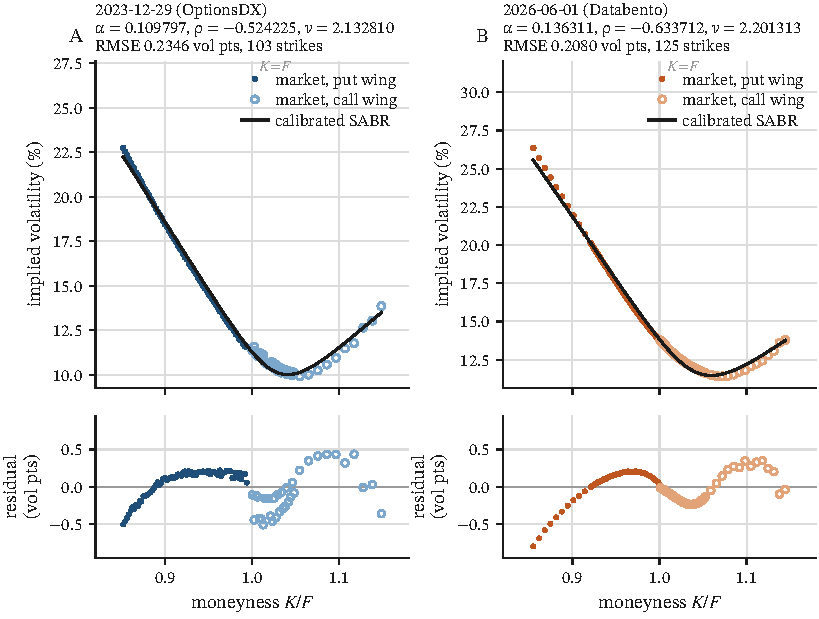
\includegraphics[width=\textwidth]{fig_sabr_fit.pdf}
\caption{Calibrated SABR against the re-implied out-of-the-money smile, plotted against
moneyness $K/F$ so that the two cases sit on a comparable axis. Solid markers are the put
wing, open markers the call wing, and the black line is \eqref{eq:hagan} evaluated at the
fitted parameters. The 2026 skew is visibly steeper --- $\hat{\rho}$ moves from
$-0.524$ to $-0.634$ --- which is legible only because the horizontal axis is shared;
against strike the two panels span \$408--\$550 and \$650--\$870 and cannot be compared
by eye. The residual panels show what the fit cannot reach. In both cases the residual
changes sign at $K=F$, which is the signature of the two wings disagreeing with each
other rather than of the model failing: fitted separately, each wing of the 2023 smile
reaches its own quote-noise floor (Section~\ref{sec:case1-sabr}).}
\label{fig:sabr}
\end{figure}

The residual pattern in Figure~\ref{fig:sabr} is a data property, not a model failure,
and establishing that is what licenses the rest of the analysis. Fitting each wing
separately and comparing the result to the strike-to-strike jitter in the quoted
volatilities themselves --- a true smile being smooth, that jitter is quote noise, and a
model that reaches it has done as well as anything could --- gives:

\begin{center}
\small
\begin{tabular}{lrrrr}
\toprule
Fit & Strikes & RMSE (vol pts) & Quote-noise floor (vol pts) & $\hat{\rho}$ \\
\midrule
Both wings & 103 & 0.2946 & 0.1140 & $-0.5108$ \\
Puts only  & 69  & \textbf{0.0751} & 0.0501 & $-0.2578$ \\
Calls only & 34  & \textbf{0.2036} & 0.1851 & $-0.6008$ \\
\bottomrule
\end{tabular}
\end{center}

\noindent (These figures are computed on the vendor's volatilities, before the correction
of Section~\ref{sec:reimply}, which is why the combined RMSE is $0.2946$ rather than
$0.2346$.) Each wing individually fits to its own noise floor. The combined fit is worse
than either because the two wings are mutually inconsistent, and the call wing is
$3.7\times$ noisier than the put wing --- SPY put quotes are simply better maintained at
end of day.

Table~\ref{tab:ident} reports the two sensitivities that justify the fixed $\beta$ and
the restricted band.

\begin{table}[t]
\centering
\small
\caption{The identification problem, made quantitative. \textbf{Upper panel:} varying the
elasticity $\beta$ across its entire admissible range moves the fit error by $0.04\vp$
while $\hat{\alpha}$ swings by a factor of 476 and $\hat{\rho}$ slides to compensate ---
the objective has a flat valley and the data cannot separate $\beta$ from $\rho$. This
is why $\beta$ is fixed rather than fitted. \textbf{Lower panel:} widening the
calibration band degrades the fit smoothly, by $2.8\times$ at the full smile, while
$\hat{\rho}$ stays within $-0.48$ to $-0.52$ throughout. The skew is well determined; it
is the wings that Hagan's asymptotic expansion cannot reach. Both panels are computed on
the 2023-12-29 chain.}
\label{tab:ident}
\begin{tabular}{lrrrrr}
\toprule
 & Strikes & RMSE (vol pts) & $\hat{\alpha}$ & $\hat{\rho}$ & $\hat{\nu}$ \\
\midrule
\multicolumn{6}{l}{\emph{Elasticity $\beta$, calibration band fixed at 15\%}}\\
$\beta=0.00$ & 103 & 0.2548 & 52.3342 & $-0.4488$ & 2.0076 \\
$\beta=0.30$ & 103 & 0.2653 &  8.2298 & $-0.4681$ & 2.0352 \\
$\beta=0.50$ & 103 & 0.2730 &  2.3979 & $-0.4807$ & 2.0542 \\
$\beta=0.70$ & 103 & 0.2813 &  0.6987 & $-0.4929$ & 2.0737 \\
$\beta=1.00$ (used) & 103 & 0.2946 & 0.1099 & $-0.5108$ & 2.1038 \\
\midrule
\multicolumn{6}{l}{\emph{Calibration band $|K/F-1|$, elasticity fixed at $\beta=1$}}\\
5\%   &  46 & 0.2040 & 0.1126 & $-0.5097$ & 1.7349 \\
10\%  &  74 & 0.2349 & 0.1117 & $-0.5198$ & 1.9425 \\
15\% (used) & 103 & 0.2946 & 0.1099 & $-0.5108$ & 2.1038 \\
20\%  & 118 & 0.3602 & 0.1086 & $-0.5033$ & 2.1887 \\
30\%  & 128 & 0.5532 & 0.1057 & $-0.4985$ & 2.3326 \\
100\% & 151 & 0.8116 & 0.0991 & $-0.4784$ & 2.5841 \\
\bottomrule
\end{tabular}
\end{table}

\subsubsection{Re-implying the volatilities}
\label{sec:reimply}

The vendor's put and call implied volatilities are mutually inconsistent. Put-call parity
requires a put and a call at the same strike to carry the same volatility; the vendor's
do not. We therefore discard them and recover every volatility ourselves, by inverting
the same BAW pricer against the same parity forward that the rest of the analysis uses.
All 151 out-of-the-money strikes inverted successfully.

The decisive evidence is the \emph{sign} of the gap at the put/call crossover. The smile
slopes downward through this strike region, so a self-consistent smile must show a
negative step going from the last put to the first call. The vendor's does not:

\begin{center}
\small
\begin{tabular}{lrrr}
\toprule
 & Last put, $K=476$ & First call, $K=479$ & Adjacent gap \\
\midrule
Vendor implied volatility & $11.379\%$ & $11.670\%$ & $+0.291\vp$ \quad(wrong sign) \\
Re-implied                & $11.567\%$ & $11.358\%$ & $-0.209\vp$ \quad(correct sign) \\
\bottomrule
\end{tabular}
\end{center}

\noindent No smooth curve can fit a kink pointing the wrong way, which is why the
combined-wing fit of Section~\ref{sec:case1-sabr} could not reach either wing's noise
floor. Panel~B of Figure~\ref{fig:reimply} shows the reversal directly. After
re-implying, the fit RMSE falls from $0.2946$ to $0.2346\vp$, the maximum error from
$0.6378$ to $0.5075\vp$, and the put-wing quote roughness from $0.0501$ to $0.0320\vp$.

\begin{figure}[t]
\centering
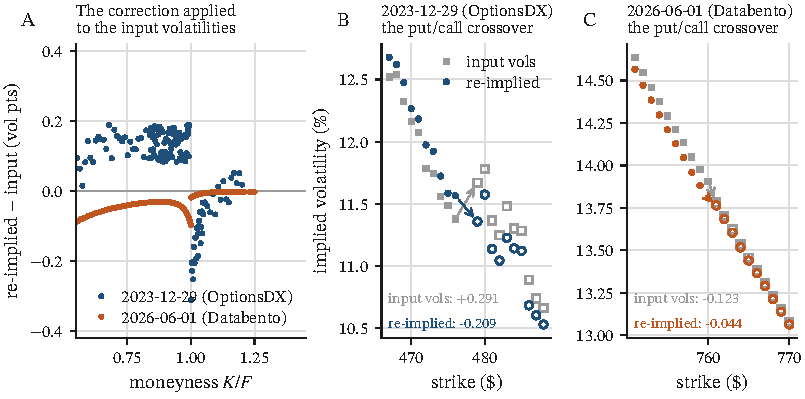
\includegraphics[width=\textwidth]{fig_reimplied.pdf}
\caption{\textbf{A:} the correction applied to the input volatilities, by moneyness. In
2023 it is a systematic offset that flips sign at the forward --- $+0.1231\vp$ on
out-of-the-money puts, $-0.0911\vp$ on calls --- which is the signature of a structural
inconsistency, not of noise. In 2026 the correction is small and one-signed
($-0.0388\vp$ across all strikes) because the input column there is this project's own
European inversion rather than a vendor's, so the panel measures the
European-to-American correction alone. \textbf{The two curves in panel A therefore do
not share a baseline and should not be read against one another:} the 2023 curve is
vendor quote error compounded with the European-to-American premium correction, while
the 2026 curve isolates that premium correction exclusively. Their relative magnitudes
say nothing about data quality. \textbf{B:} the 2023 put/call crossover. The grey
arrow is the vendor's step, $+0.291\vp$, pointing \emph{upward} against a downward-sloping
smile --- a shape no smooth curve can fit. The blue arrow is the same step after
re-implying, $-0.209\vp$, correctly signed. \textbf{C:} the same construction in 2026,
where both the pre- and post-correction gaps already carry the correct negative sign. An
internally consistent starting point does not produce the kink.}
\label{fig:reimply}
\end{figure}

\subsubsection{The BAW pricer and what the approximation costs}
\label{sec:baw-results}

The pricer was built and validated with no involvement from the smile model: volatility
is a plain input argument here. Table~\ref{tab:baw} lists the ten checks. Correctness
rests on the exact structural properties --- tests 1, 2, 3, 7 and 8, all of which hold to
machine precision or better --- and not on the approximation-quality comparisons, which
measure the accuracy of the \emph{method} rather than of the implementation.

\begin{table}[t]
\centering
\small
\caption{The BAW validation suite. Tests 1--3 and 7--8 are exact structural properties and
establish implementation correctness; tests 4--6 measure the accuracy of the
approximation itself and are reported rather than asserted. No benchmark table was
transcribed from the original paper: reference values that could not be verified from
the build environment would validate the pricer against fiction, so the reference is a
convergent Cox-Ross-Rubinstein lattice \citep{crr1979}, which is the method
Barone-Adesi and Whaley used to assess their own approximation. Test~2 is the sharpest
single check of a BAW implementation and it passes to \emph{exactly} zero rather than to
tolerance.}
\label{tab:baw}
\begin{tabular}{rlp{0.50\textwidth}}
\toprule
\# & Check & Result \\
\midrule
1 & European put-call parity & worst error $2.8\times10^{-14}$ across 6 cases \\
2 & American call $=$ European when $b=r$ & worst spurious premium \textbf{exactly} $0.0$, 5 cases \\
3 & American $\ge$ European and $\ge$ intrinsic & 0 violations in 1{,}350 grid points \\
4 & BAW vs.\ lattice, stress grid & worst absolute error \$0.0599 (tolerance \$0.10) \\
5 & BAW vs.\ lattice, SPY regime & worst absolute error \$0.1439 (tolerance \$0.20) \\
6 & P\&L error propagation & informational; see text \\
7 & Monotonicity in $S$, $\sigma$, $T$ & 10 sequences, all correct \\
8 & Critical exercise prices & correct side of strike, recede as $\sigma$ rises \\
9 & Implied-volatility round trip & 128 cases, worst error $7.893\times10^{-6}$ \\
10 & SPY reference case & informational \\
\bottomrule
\end{tabular}
\end{table}

Two properties of the approximation constrain everything downstream, and
Figure~\ref{fig:baw} shows both.

\emph{Calls are exact in the 2023 regime.} With $b=5.5926\%>r=5.4000\%$, early exercise
on a call is never optimal, \eqref{eq:critical} has no finite solution, the pricer
returns the European value and the lattice agrees to $0.02\%$. There is no premium to get
wrong. This is precisely why the reference position is a put: a call would exercise none
of the American machinery.

\emph{Puts carry a real error whose sign flips with moneyness.} At the reference expiry,
BAW recovers about $95\%$ of the at-the-money put's early-exercise premium (\$0.2914
against a true \$0.3069) while \emph{overstating} it out of the money by more than a
factor of two (\$0.0362 against \$0.0167). The absolute errors are small --- \$0.0155 at
the money, \$0.0195 at $K=450$ --- and the large relative error out of the money is an
artefact of a small denominator.

\begin{figure}[t]
\centering
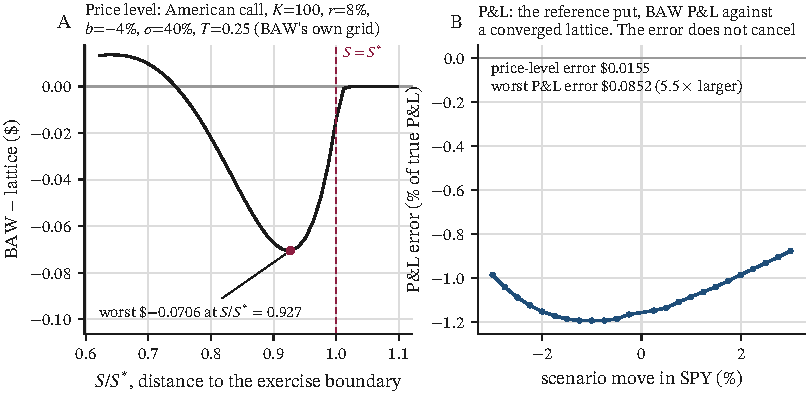
\includegraphics[width=\textwidth]{fig_baw_accuracy.pdf}
\caption{What the quadratic approximation costs. \textbf{A:} BAW minus a converged
8{,}000-step lattice for an American call on the parameter set Barone-Adesi and Whaley
use for their own accuracy tables, plotted against distance to the exercise boundary
$S^{*}$. The error is near zero at the money, peaks at $-\$0.0706$ at $S/S^{*}=0.927$ ---
just below the boundary, where the term dropped from the pricing equation matters most
--- and is exactly zero beyond it, where the option is worth its intrinsic value. This is
the approximation's documented weakness, not a defect: it is why the validation
tolerances in Table~\ref{tab:baw} are set on absolute dollar error rather than relative
error. (A five-point grid over the same parameters reports the peak as \$0.0700 at
$S/S^{*}=0.915$; the finer sampling here locates it slightly differently.) \textbf{B:}
the consequence for a risk number. Scenario P\&L is a \emph{difference} of two prices at
two different spots, and because BAW's error varies with spot and changes sign with
moneyness, it does not cancel in that difference --- it survives at approximately $-1\%$
of the true P\&L across the entire range of daily moves a 250-day SPY sample contains.
The worst P\&L error, \$0.0852, is $5.5\times$ the \$0.0155 price-level error.}
\label{fig:baw}
\end{figure}

The consequence for the risk number is Panel~B of Figure~\ref{fig:baw}, and it is the
opposite of what one might assume. It would be comfortable to expect the pricing error
to cancel in the scenario-minus-base subtraction, since the same systematic bias sits in
both terms. It does not. Because the error varies with spot and changes sign with
moneyness, differencing two prices at two different spots leaves \emph{more} error than
either price carried alone: the worst P\&L error of \$0.0852 is $5.5\times$ the
price-level error of \$0.0155. \textbf{Approximately $1\%$ of every scenario P\&L, and
therefore of the final VaR, is an artefact of using BAW rather than a lattice.} The
filing specifies BAW, so this is the intended behaviour rather than an error, but it is
a real precision floor and it is not removable within the specification.

\subsubsection{The SABR-to-BAW junction}
\label{sec:junction}

The two models meet at a single point: the curve is read at the \emph{forward} and the
pricer is called from \emph{spot}. Conflating the two is the classic error at this
junction, and here they differ by \$3.58, more than three strike increments. Pricing all
103 calibration strikes through the joined models against the market gives a mean
absolute error of \$0.0718 and a mean \emph{signed} error of $-\$0.0007$: scatter without
bias.

Only 6 of 103 theoretical prices land inside the quoted bid-ask spread, which looks
alarming until the spreads are examined --- the median SPY spread here is \$0.010, less
than $1\%$ of mid, so ``inside the spread'' demands matching the market to half a cent,
a standard no smile model meets. Absolute error is the meaningful measure.

The test that matters is attribution. If the wiring were wrong --- spot passed where the
forward belongs, a mismatched day count, an incorrect carry --- the resulting error would
be structural and would not track the volatility fit error. Multiplying each strike's
volatility error by its vega and comparing predicts the observed pricing error almost
exactly (Figure~\ref{fig:attrib}): $99.21\%$ of the error is explained, with a
correlation of $0.999974$ and a mean unexplained residual of \$0.000567. Vega is computed
here for attribution only and is never used to price a scenario.

\begin{figure}[t]
\centering
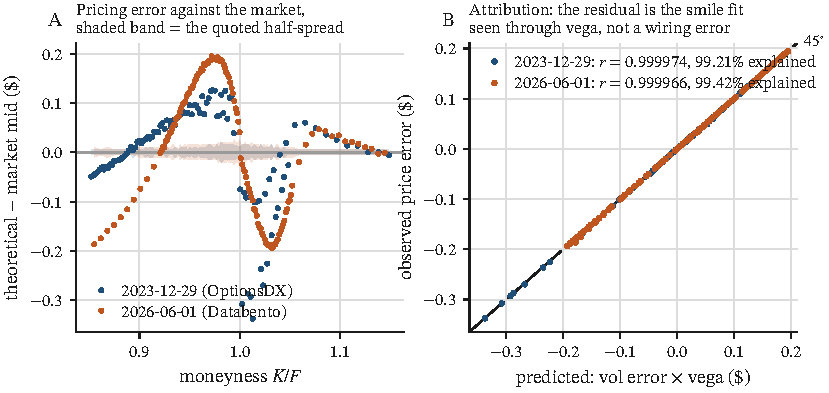
\includegraphics[width=\textwidth]{fig_price_attribution.pdf}
\caption{\textbf{A:} theoretical price minus market mid across the calibration band, with
the quoted half-spread shaded. The errors are an order of magnitude larger than the
spread --- SPY spreads here have a median of \$0.010 --- so ``inside the spread'' is not
an achievable standard for a smile model and absolute error is the meaningful measure.
The oscillating shape is the SABR residual of Figure~\ref{fig:sabr} seen through vega.
\textbf{B:} the attribution test. Each strike's observed pricing error is plotted against
the error predicted from its volatility fit error multiplied by its vega. The points lie
on the $45^{\circ}$ line: $99.21\%$ and $99.42\%$ of the pricing error is explained in
the two cases, with correlations of $0.999974$ and $0.999966$. A wiring error --- spot
passed where the forward belongs, a mismatched day count, a wrong carry --- would be
structural and would not track the volatility fit. It does track it, so what remains is
the smile fit, which is limited by the data rather than by the plumbing.}
\label{fig:attrib}
\end{figure}

\subsubsection{Scenarios and full revaluation}

The 250 scenarios are drawn from 2023-01-03 to 2023-12-29 --- exactly calendar 2023, since
250 sessions back from the reference date lands on the first trading day of the year ---
and produce scenario spot prices from \$465.80 to \$486.16. The window contains zero
calendar defects. Its statistics appear in Table~\ref{tab:windows}.

Three sanity checks on the revaluation loop pass. A scenario with a $+0.0000\%$ return
reprices to the base price with a P\&L of exactly \$0.000000. P\&L is monotone in the
underlying move across all 250 scenarios, as a long put requires. And the P\&L is convex:
symmetric up and down moves of $0.5\%$, $1\%$, $2\%$ and $3\%$ sum to $+0.1221$,
$+0.4899$, $+1.9815$ and $+4.5188$ respectively, where a linear position would sum to
exactly zero on every row. That convexity is the entire reason full revaluation is
required, and Figure~\ref{fig:reval} shows what ignoring it would cost.

\begin{figure}[t]
\centering
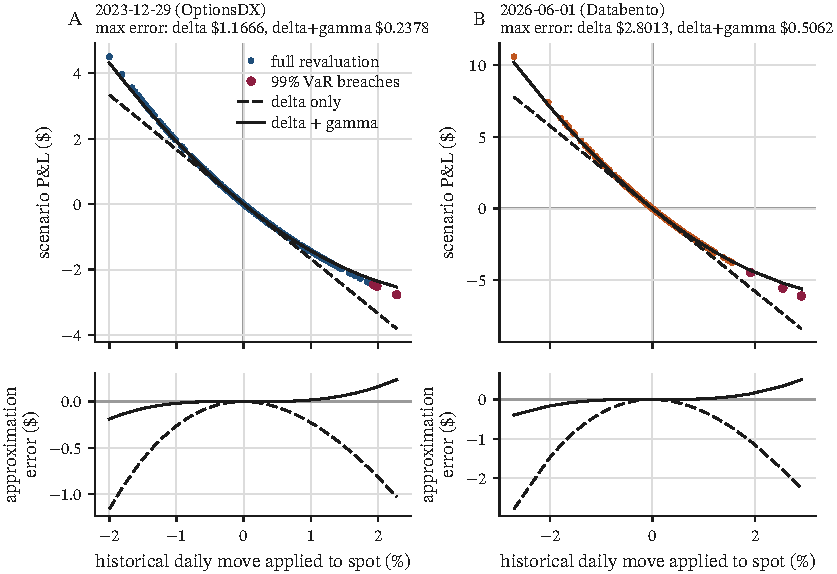
\includegraphics[width=\textwidth]{fig_full_revaluation.pdf}
\caption{The filing's prohibition, priced. Points are fully revalued scenario P\&Ls; the
lines are the delta-only and delta-plus-gamma expansions of \eqref{eq:taylor}, computed
with Greeks taken from the full chain including the smile's response to spot --- that is,
the most favourable version of the shortcut available. The lower panels show the
approximation error directly. Delta alone is wrong by up to \$1.17 in the 2023 case,
$17.6\%$ of the whole \$6.64 position value. Delta plus gamma is much better but fails
where it matters: on the single worst 2023 scenario it returns $-\$2.534$ against a true
$-\$2.772$, \emph{understating} the worst-case loss by $8.6\%$. Note also that every VaR
breach (wine) lies on the \emph{right}: a long put loses when the market rallies, so the
scenarios driving this VaR are the best days of the year, not the worst.}
\label{fig:reval}
\end{figure}

\subsubsection{Value-at-Risk}
\label{sec:case1-var}

Applying \eqref{eq:rank} and \eqref{eq:var} to the 250 scenario P\&Ls gives a $99\%$
one-day VaR of \textbf{\$2.4488} and an expected shortfall of \textbf{\$2.5805}, or
$36.89\%$ and $38.87\%$ of the \$6.6391 position value. The arithmetic, reproduced in
full in Table~\ref{tab:var}, is deliberately transparent: the fractional rank
$h=(250-1)\times0.01=2.49$ falls between the third and fourth worst scenarios, and the
quantile is their weighted blend.

An independent recomputation with \texttt{numpy.percentile} using the linear method
agrees to $0.000\times10^{0}$ --- it returns $-2.448845174615$ against our
$-2.448845174615$. The agreement is exact because NumPy's default uses the same
$(N-1)p$ rank definition we implemented, which is precisely why it is a good check on the
arithmetic and a poor substitute for the implementation: calling it would have meant
adopting whichever convention the library happens to default to rather than stating one.

\subsection{Case 2: 2026-06-01, Databento}
\label{sec:case2}

The same code was run against the Databento-sourced dataset with only the configuration
changed. Every stage behaved, and in two respects behaved better than on the original
data.

All 197 out-of-the-money strikes inverted successfully, none failed. The SABR fit is
\emph{better} than on the original chain, with an RMSE of $0.2080\vp$ over 125 strikes
against $0.2346$ over 103 --- evidence that the pipeline is not overfitted to the inputs
it was developed on. The attribution test of Section~\ref{sec:junction} gives $99.42\%$
explained with a correlation of $0.999966$, essentially reproducing the first case's
result on independent data.

Three features of the market state differ materially and are worth stating before the
risk numbers, because they are what the risk numbers reflect.

\textbf{The carry regime flips.} The implied dividend yield is $+1.8999\%$ against
$-0.1926\%$ in 2023. This is a calendar fact rather than a modelling artefact: one SPY
ex-dividend date falls between 2026-06-01 and 2026-07-17 where none fell in the 2023
window. Stated in dollars rather than annualised, $+1.8999\%$ is \$1.82 of dividend on a
\$758.54 underlying, which is SPY's actual quarterly payout. Nothing in the calibration
forces this; it falls out of put-call parity applied to the quotes. The consequence runs
through the pricing: with $b<r$ an American call now \emph{does} carry early-exercise
value, and the put's premium is larger here than in the first case, so the choice of a
put as the reference position holds for the opposite reason.

\textbf{Rates fell}, $5.40\%$ to $3.66\%$, pinned externally from the same FRED series in
both cases.

\textbf{The skew steepened and the volatility level rose} --- $\hat{\rho}$ from $-0.524$
to $-0.634$, at-the-money implied volatility from $11.76\%$ to $13.94\%$ --- against
\emph{lower} realised volatility in the lookback window, $13.14\%$ to $11.88\%$. A higher
implied volatility on a calmer realised window is a genuine feature of the 2026 surface.

The resulting $99\%$ one-day VaR is \textbf{\$4.1216} with an expected shortfall of
\textbf{\$5.3674}, or $28.58\%$ and $37.22\%$ of the \$14.4221 position value. The full
arithmetic is in Table~\ref{tab:var} and the distribution in Figure~\ref{fig:pnl}.

\begin{table}[t]
\centering
\small
\caption{Value-at-Risk and expected shortfall for both cases, with the interpolation of
\eqref{eq:rank}--\eqref{eq:var} reproduced in full so that each figure can be rebuilt by
hand. In both cases the fractional rank $h=2.49$ falls between the third and fourth worst
scenarios and the quantile is their weighted blend. Note that every bracketing scenario
is an \emph{up} day: a long put loses when the market rallies. The stress rows apply the
same position and the same calibrated surface to a harsher return window, changing only
the return distribution; they should be read as upper bounds for the reason given in
Section~\ref{sec:limitations}.}
\label{tab:var}
\begin{tabular}{lrrrr}
\toprule
 & \multicolumn{2}{c}{2023-12-29} & \multicolumn{2}{c}{2026-06-01} \\
\cmidrule(lr){2-3}\cmidrule(lr){4-5}
 & Baseline & Stress (2020) & Baseline & Stress (to 2026-01-02) \\
\midrule
Scenarios $N$              & 250 & 250 & 250 & 250 \\
Tail probability $p$       & 0.01 & 0.01 & 0.01 & 0.01 \\
Fractional rank $h=(N-1)p$ & 2.49 & 2.49 & 2.49 & 2.49 \\
Lower order statistic $L_{(3)}$ (\$) & $-2.462080$ & $-5.052603$ & $-4.459823$ & $-5.631089$ \\
Upper order statistic $L_{(4)}$ (\$) & $-2.435070$ & $-4.806637$ & $-3.769542$ & $-4.797515$ \\
Interpolation weight $w$   & 0.49 & 0.49 & 0.49 & 0.49 \\
Interpolated quantile $\hat{Q}$ (\$) & $-2.448845$ & $-4.932080$ & $-4.121585$ & $-5.222638$ \\
\midrule
\textbf{99\% one-day VaR} (\$) & \textbf{2.4488} & \textbf{4.9321} & \textbf{4.1216} & \textbf{5.2226} \\
\quad as \% of position value  & 36.89 & 74.29 & 28.58 & 36.21 \\
Expected shortfall (\$)        & 2.5805 & 5.3881 & 5.3674 & 8.0276 \\
\quad breaching scenarios      & 3 & 3 & 3 & 3 \\
Worst scenario P\&L (\$)       & $-2.7719$ & $-5.5885$ & $-6.0986$ & $-11.7889$ \\
\quad produced by              & 2023-01-06 & 2020-03-13 & 2026-03-31 & 2025-04-09 \\
\quad that day's SPY move      & $+2.283\%$ & $+9.290\%$ & $+2.907\%$ & $+10.502\%$ \\
Stress $/$ baseline            & --- & $2.01\times$ & --- & $1.27\times$ \\
Position value $V_0$ (\$)      & 6.6391 & 6.6391 & 14.4221 & 14.4221 \\
\bottomrule
\end{tabular}
\end{table}

\begin{figure}[t]
\centering
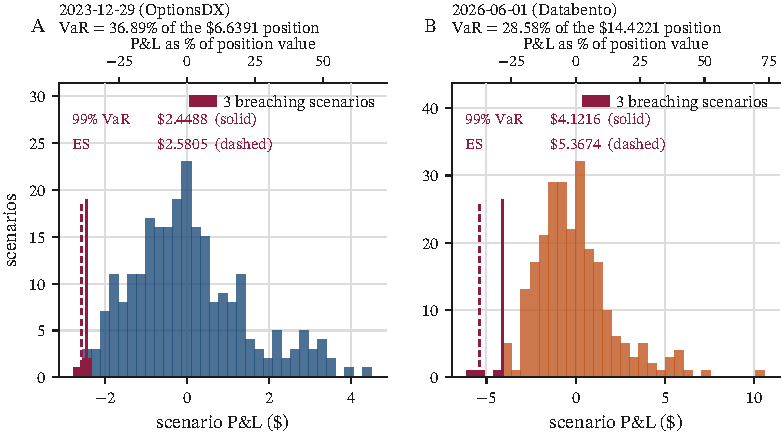
\includegraphics[width=\textwidth]{fig_pnl_distribution.pdf}
\caption{The fully revalued scenario P\&L distributions, with the interpolated $99\%$
threshold (solid) and expected shortfall (dashed) marked and the three breaching
scenarios in wine. The secondary axis expresses P\&L as a percentage of position value,
which is the only like-for-like comparison between the two cases: the dollar figures are
not comparable because the positions differ in strike and in underlying level. On that
basis the 2026 case is the \emph{less} risky of the two, $28.58\%$ against $36.89\%$.
Both distributions are right-skewed, which is gamma: a long option gains more from a
large move than it loses from a move of the same size in the other direction. The 2026
distribution has the visibly longer right tail, consistent with its window's excess
kurtosis of $+1.569$ against $-0.178$.}
\label{fig:pnl}
\end{figure}

\subsection{The two cases compared}
\label{sec:staged}

Table~\ref{tab:staged} sets the two runs side by side. They disagree substantially, and
the question worth answering is whether the disagreement is the market or the plumbing.

\begin{table}[t]
\centering
\small
\caption{The two reference cases side by side. The dollar VaRs are not directly
comparable --- different strikes on a different underlying level, and marginally
different moneyness sign --- so VaR as a percentage of position value is the like-for-like
figure, and on that basis the second case is the less risky of the two. The upper block
lists differences attributable to the market; the lower block bounds what the change of
data source could contribute, measured on a shared date by the cross-vendor check of
Section~\ref{sec:crossvendor}.}
\label{tab:staged}
\begin{tabular}{lrr}
\toprule
 & 2023-12-29 (OptionsDX) & 2026-06-01 (Databento) \\
\midrule
\multicolumn{3}{l}{\emph{Market state}}\\
Risk-free rate $r$            & 5.4000\% & 3.6600\% \\
Cost of carry $b$             & 5.5926\% & 1.7601\% \\
Implied dividend yield $q$    & $-0.1926\%$ & $+1.8999\%$ \\
Carry regime                  & $b>r$ & $b<r$ \\
SABR $\hat{\rho}$ (skew)      & $-0.524225$ & $-0.633712$ \\
At-the-money implied volatility & 11.76\% & 13.94\% \\
Fit RMSE                      & $0.2346\vp$ & $0.2080\vp$ \\
\midrule
\multicolumn{3}{l}{\emph{Lookback window}}\\
Realised volatility (annualised) & 13.14\% & 11.88\% \\
Skewness                      & $-0.028$ & $-0.244$ \\
Excess kurtosis               & $\mathbf{-0.178}$ & $\mathbf{+1.569}$ \\
Worst / best day              & $-2.00\%$ / $+2.28\%$ & $-2.70\%$ / $+2.91\%$ \\
\midrule
\multicolumn{3}{l}{\emph{Result}}\\
Position value (\$)           & 6.6391 & 14.4221 \\
\textbf{99\% one-day VaR} (\$) & \textbf{2.4488} & \textbf{4.1216} \\
\textbf{VaR as \% of position} & \textbf{36.89\%} & \textbf{28.58\%} \\
Expected shortfall (\$)       & 2.5805 & 5.3674 \\
Stress $/$ baseline           & $2.01\times$ & $1.27\times$ \\
\midrule
\multicolumn{3}{l}{\emph{Data-source contribution, measured on the shared date 2023-12-29}}\\
Median mid price difference   & \multicolumn{2}{c}{\$0.0000 over 151 strikes} \\
Median re-implied IV difference & \multicolumn{2}{c}{$0.0000\vp$} \\
95th percentile $|$IV difference$|$ & \multicolumn{2}{c}{$0.2286\vp$} \\
Parity forward difference     & \multicolumn{2}{c}{$-\$0.0425$ \ (0.89 bp)} \\
Re-implied crossover gap      & \multicolumn{2}{c}{reproduced to $0.0076\vp$} \\
\bottomrule
\end{tabular}
\end{table}

It is the market. Set against differences of $68\%$ in dollar VaR and $8.3$ percentage
points in VaR-to-position, a forward that agrees between vendors to $0.89$ basis points
and implied volatilities whose median difference is exactly zero cannot be carrying the
result. The sharpest single regime difference is the shape of the tails: the 2023 window
has excess kurtosis of $-0.178$, meaning tails \emph{thinner} than a normal distribution,
while the 2026 window has $+1.569$. Both windows are calm by their own volatility
measure; the second is calm in a fat-tailed way.

One asymmetry should be stated rather than glossed. The stress ratios, $2.01\times$ and
$1.27\times$, are not comparable to each other. The first case's dataset reaches 2020;
the Databento pull spans seventeen months, so the harshest window available to the second
case is the one containing the April 2025 selloff. That is a smaller multiple because
April 2025 was a smaller event than March 2020, not because the method behaved
differently.

\subsection{The lookback window dominates the answer}
\label{sec:window}

The largest sensitivity in this study is not a modelling choice. It is which twelve
months precede the reference date.

Evaluating the same position by the same method as if standing at the end of each of
several past years gives the upper block of Table~\ref{tab:windows}. The 2023 window is
the calmest of six by a wide margin and the only one with negative excess kurtosis; every
other window shows the textbook fat tails. Its first percentile return, which is
essentially what a $99\%$ VaR reads, is $-1.64\%$ against $-6.76\%$ for a window ending
in 2020 --- a factor of $4.1$. That factor is neither a modelling choice nor a market
view.

\begin{table}[t]
\centering
\small
\caption{Return-window statistics. \textbf{Upper block:} the 2023 case's window against
five earlier year-end windows from the same dataset. Ours is the calmest of the six and
the only one with negative excess kurtosis --- not one day in calendar 2023 moved beyond
three standard deviations, against the $0.67$ such days a fitted normal predicts, so the
tails are \emph{thinner} than normal rather than fatter. (These comparison years are
context only and are not put through the calendar validation of Section~\ref{sec:data};
vendor data quality varies by year, and the reference window itself is clean.)
\textbf{Lower block:} the 2026 case's window against four earlier reference dates from
within the same continuous seventeen-month dataset. The first percentile holds at
$-3.56\%$ for three successive dates and then halves to $-1.75\%$, because the April 2025
selloff leaves the 250-day window between them.}
\label{tab:windows}
\begin{tabular}{lrrrrr}
\toprule
As of & Ann.\ vol & Skewness & Excess kurtosis & Worst day & 1st percentile \\
\midrule
\multicolumn{6}{l}{\emph{OptionsDX dataset, year-end windows}}\\
2011-12-30 & 23.08\% & $-0.433$ & $+2.581$ & $-6.51\%$ & $-4.34\%$ \\
2015-12-31 & 15.65\% & $-0.231$ & $+2.117$ & $-4.13\%$ & $-2.78\%$ \\
2018-12-31 & 17.18\% & $-0.409$ & $+3.148$ & $-4.21\%$ & $-3.21\%$ \\
2020-12-31 & 34.14\% & $-0.598$ & $+7.631$ & $-11.51\%$ & $-6.76\%$ \\
2022-12-30 & 24.09\% & $+0.026$ & $+0.362$ & $-4.34\%$ & $-3.74\%$ \\
\textbf{2023-12-29} (Case 1) & \textbf{13.14\%} & $\mathbf{-0.028}$ & $\mathbf{-0.178}$ & $\mathbf{-2.00\%}$ & $\mathbf{-1.64\%}$ \\
\midrule
\multicolumn{6}{l}{\emph{Databento dataset, rolling reference dates}}\\
2026-01-02 & 19.48\% & $+1.514$ & $+23.636$ & $-5.85\%$ & $-3.56\%$ \\
2026-01-30 & 19.30\% & $+1.555$ & $+24.644$ & $-5.85\%$ & $-3.56\%$ \\
2026-03-16 & 18.88\% & $+1.703$ & $+26.960$ & $-5.85\%$ & $-3.56\%$ \\
2026-04-28 & 12.51\% & $+0.068$ & $+2.067$  & $-2.70\%$ & $-1.75\%$ \\
\textbf{2026-06-01} (Case 2) & \textbf{11.88\%} & $\mathbf{-0.244}$ & $\mathbf{+1.569}$ & $\mathbf{-2.70\%}$ & $\mathbf{-1.75\%}$ \\
\bottomrule
\end{tabular}
\end{table}

The lower block of Table~\ref{tab:windows} makes the same point more directly, because it
holds the dataset, the vendor and the underlying fixed and moves only the reference date.
The April 2025 tariff selloff ($-5.85\%$, followed five sessions later by $+10.50\%$)
sits at sessions 63--68 of the Databento pull. It is inside the 250-day window for
reference dates up to roughly 2026-03 and has aged out by 2026-04-28. Across that
boundary the window's first percentile halves, from $-3.56\%$ to $-1.75\%$, its annualised
volatility falls from $18.88\%$ to $12.51\%$ and its excess kurtosis collapses from
$+26.96$ to $+2.07$. Nothing about the market changed at that moment. Only the window
did. Figure~\ref{fig:window} shows both effects.

\begin{figure}[t]
\centering
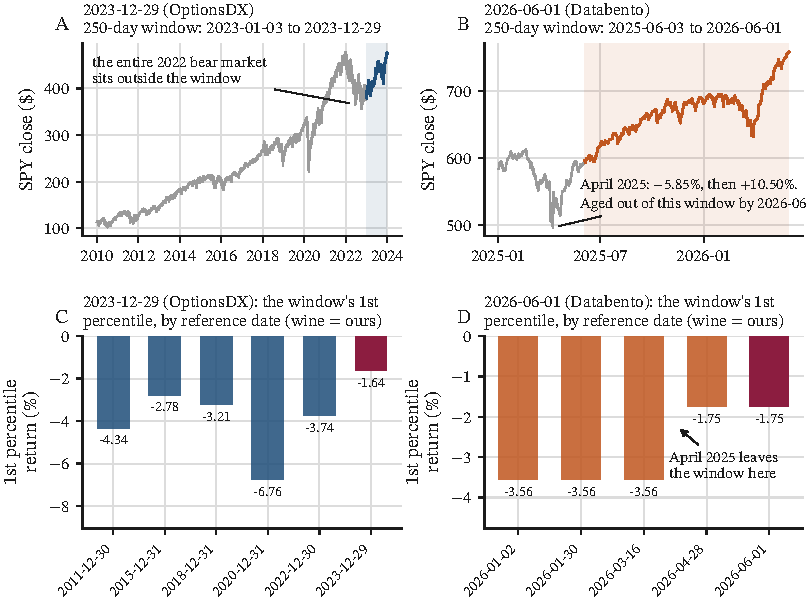
\includegraphics[width=\textwidth]{fig_lookback_window.pdf}
\caption{The dominant sensitivity in the study. \textbf{A, B:} the SPY price path for each
dataset with the 250-day lookback window shaded. In the 2023 case the entire 2022 bear
market --- which took SPY from \$477 to \$357 --- sits outside the window and contributes
nothing to the VaR. In the 2026 case the April 2025 selloff sits just outside the shaded
region for the same reason. \textbf{C, D:} the window's first-percentile return as the
reference date moves, same position and same method throughout. Panel~D is the sharper
demonstration because it holds the dataset, the vendor and the underlying fixed: the
first percentile is unchanged at $-3.56\%$ for three successive reference dates and then
halves to $-1.75\%$, purely because April 2025 has fallen off the back of the window.
This is the central weakness of unweighted historical simulation --- a crisis counts
fully until the day it leaves the window, and not at all afterwards.}
\label{fig:window}
\end{figure}

% ============================================================ 5. ROBUSTNESS
\section{Robustness and diagnostics}
\label{sec:robustness}

\subsection{The put/call inconsistency: what was an artefact and what was not}
\label{sec:crossover}

Section~\ref{sec:reimply} showed that re-implying the volatilities removed a
wrong-signed kink at the put/call crossover and improved the fit. It did not remove the
inconsistency entirely, and the cross-vendor data of Section~\ref{sec:crossvendor} allows
the remainder to be separated into a vendor artefact and a market feature.

\paragraph{The kink was the vendor's.} The OptionsDX volatilities stepped $+0.291\vp$
upward across a downward-sloping smile. Databento does not reproduce this. Relatedly,
the two crossed put quotes at $K=477$ and $K=478$ (bid 7.36 / ask 7.33, and bid 7.78 /
ask 7.77) that forced those strikes out of the OptionsDX smile are clean and two-sided in
the Databento data (7.37 / 7.40 and 7.80 / 7.83), which contains zero crossed quotes in
the entire out-of-the-money chain. Both were vendor defects. The second reference case
corroborates this independently: in 2026 both the pre-correction and post-correction gaps
carry the correct negative sign ($-0.1227$ and $-0.0436$), so an internally consistent
starting point does not produce the kink.

\paragraph{The residual is real.} Measuring the crossover anomaly as the adjacent gap
minus what the put wing's own slope predicts, using a slope fitted over a range of
strikes rather than a two-point difference:

\begin{center}
\small
\begin{tabular}{lrrrr}
\toprule
 & Adjacent gap & Fitted wing slope & Predicted gap & Residual \\
\midrule
OptionsDX, $476\to479$ (\$3 span)   & $-0.2088$ & $-0.1264$/\$1 & $-0.3792$ & $+0.1704$ \\
Databento, $476\to479$ (\$3 span)   & $-0.2164$ & $-0.1287$/\$1 & $-0.3860$ & $+0.1697$ \\
Databento, $478\to479$ (\$1 span)   & $+0.0208$ & $-0.1254$/\$1 & $-0.1254$ & $+0.1462$ \\
\bottomrule
\end{tabular}
\end{center}

\noindent All quantities in volatility points. The two vendors agree on identical strikes
to $0.0007\vp$, and closing the \$3 gap left by the crossed OptionsDX quotes --- possible
only in the Databento data --- moves the answer by $0.024$. \textbf{The residual put/call
inconsistency is a genuine market feature of roughly $+0.15\vp$, not a vendor artefact.}

We tested two explanations and neither closes it. It is not the forward: the gap would
vanish at $F\approx\$479.6$, some \$0.70 above the parity forward and $3.5$ standard
deviations of that estimate, so not noise. Correcting the known European-for-American
bias in \eqref{eq:parity} --- subtracting each leg's early-exercise premium before
applying parity --- moves the forward from \$478.892 to \$479.036, which is
$+\$0.144$, about $20\%$ of the gap. The bias is real and correctly signed but it is not
the main cause. The most likely remainder is that the parity forward is computed from
both legs, one of which is always the illiquid in-the-money one. We report this as
unresolved.

\paragraph{A diagnostic of ours that the second source falsified.} This is worth
recording because it is a negative result about our own instrument, not about the data.
Our crossover diagnostic originally predicted the expected gap from a \emph{two-point}
local slope --- the last two put quotes only --- a choice made deliberately to keep the
measure local. On this date that choice fails:

\begin{center}
\small
\begin{tabular}{lrrr}
\toprule
 & Two-point slope & Predicted gap & Residual \\
\midrule
OptionsDX, $476\to479$ & $-0.0193$/\$1 & $-0.0578$ & $\mathbf{-0.1510}$ \\
Databento, $476\to479$ & $-0.1084$/\$1 & $-0.3253$ & $\mathbf{+0.1089}$ \\
Databento, $478\to479$ & $-0.1126$/\$1 & $-0.1126$ & $+0.1334$ \\
\bottomrule
\end{tabular}
\end{center}

\noindent The residual \emph{changes sign between vendors on the same strikes}. The cause
is a single quote: the $475\to476$ put volatility step is $-0.0193\vp$ in the OptionsDX
data against $-0.1084\vp$ in Databento, because the OptionsDX \$475 put mid is seven
cents low. A two-point slope has no averaging, so a one-cent quote error propagates
undamped --- here it flattened the slope by a factor of $5.6$ and flipped the sign of the
conclusion. The fitted-slope measure is stable across vendors ($+0.1704$ against
$+0.1697$) and across strike pairs, and is the measure the paragraph above uses. Any
figure computed from the two-point version, including one we previously recorded, should
not be relied upon.

\subsection{The rank convention is a larger ambiguity than the first case suggests}
\label{sec:rank}

The filing's phrase ``linear interpolation to the $99\%$ threshold'' does not determine a
calculation, because it leaves open where in index space the threshold sits.
Table~\ref{tab:rank} recomputes both cases' VaR under the three conventions in common use.

\begin{table}[t]
\centering
\small
\caption{Sensitivity of the reported VaR to the quantile rank convention of
\eqref{eq:rank}. All three are in common use and the filing specifies none of them
\citep{hyndman1996}. In the first case the ambiguity is worth $1.46\%$ of the VaR, small
enough to be dismissed. In the second it is worth $21.26\%$, because the Weibull rank of
$1.51$ lands between the second and third worst scenarios of a fat-tailed sample where
the first case's thin-tailed sample is nearly flat. The wording's indeterminacy is
therefore not a fixed small quantity but one that scales with the shape of the tail ---
which is precisely the regime in which a margin figure matters most.}
\label{tab:rank}
\begin{tabular}{lrrrr}
\toprule
 & \multicolumn{2}{c}{2023-12-29} & \multicolumn{2}{c}{2026-06-01} \\
\cmidrule(lr){2-3}\cmidrule(lr){4-5}
Convention & Rank $h$ & VaR (\$) & Rank $h$ & VaR (\$) \\
\midrule
$(N-1)p$ \ \ (R type 7, NumPy default, \textbf{ours}) & 2.4900 & 2.4488 & 2.4900 & 4.1216 \\
$Np$                                                  & 2.5000 & 2.4486 & 2.5000 & 4.1147 \\
$(N+1)p-1$ \ \ (R type 6, Weibull)                    & 1.5100 & 2.4844 & 1.5100 & 4.9909 \\
\midrule
Spread across conventions (\$)                        & \multicolumn{2}{c}{0.0358} & \multicolumn{2}{c}{0.8762} \\
\quad as \% of the reported VaR                       & \multicolumn{2}{c}{\textbf{1.46\%}} & \multicolumn{2}{c}{\textbf{21.26\%}} \\
\bottomrule
\end{tabular}
\end{table}

Reporting only the first case would have supported the comfortable conclusion that the
convention barely matters. It does not generalise. At $N=250$ the three ranks differ by
at most one position in the order statistics, so the spread is governed entirely by how
steep the P\&L distribution is between the second and fourth worst scenarios --- nearly
flat in the thin-tailed 2023 sample, steep in the fat-tailed 2026 one. The ambiguity also
grows as the scenario count falls. A specification that intends a reproducible number
must name the convention.

\subsection{The cost of the approximations, collected}

Three sources of error have been measured rather than assumed, and it is worth setting
them beside one another because they are of very different sizes.

The BAW approximation contributes approximately $1\%$ to every scenario P\&L
(Section~\ref{sec:baw-results}), amplified $5.5\times$ from the price level because its
sign changes with moneyness. It is not removable within the specification, since the
filing names BAW; a converged lattice would remove it at roughly a thousandfold increase
in runtime.

The rank convention contributes $1.46\%$ or $21.26\%$ depending on the case
(Section~\ref{sec:rank}). It is removable at zero cost by naming a convention.

The data source contributes a median of exactly zero (Section~\ref{sec:crossvendor}),
with a 95th-percentile implied-volatility difference of $0.2286\vp$ and a forward
agreeing to $0.89$ basis points.

Against these, the lookback window moves the first-percentile return by a factor of
$4.1$ across the windows in Table~\ref{tab:windows}, and by a factor of $2.0$ within a
single continuous dataset over four months. The ordering is not close.

% ============================================================ 6. LIMITATIONS
\section{Limitations}
\label{sec:limitations}

The following bound what these results establish. Several are consequences of matching
the filing rather than defects, and are marked as such.

\textbf{Neither lookback window contains a crisis.} This is the dominant limitation and
it is quantified in Section~\ref{sec:window}. Calendar 2023 had realised volatility of
$13.14\%$, excess kurtosis of $-0.178$ and not one day beyond three standard deviations;
its first percentile return is $-1.64\%$ against $-6.76\%$ for a window ending in 2020.
Both reported VaRs are benign as a consequence of their windows, not of their positions.
The unweighted window is specified by the filing, so this is intended behaviour, but it
means neither number should be read as an estimate of what the position could lose in a
stressed market.

\textbf{There is no independent volatility risk in either number.} The surface is frozen
at its reference calibration and only the anchor point moves with spot, so scenario P\&L
contains spot risk and the smile's response to spot and nothing else. For a long option
this matters a great deal. On the worst 2020 stress scenario --- a $+9.29\%$ day --- the
frozen surface gives a loss of \$5.59; lifting volatility by ten points cuts that to
\$1.90 and by twenty points turns it into a \$3.32 gain. A genuine joint replay would
shock the surface with the same historical day's surface, and the historical surfaces to
build that do exist in the dataset. It was not built.

\textbf{The stress figures are therefore upper bounds, in a direction that must be stated
explicitly.} A long put is long vega and loses on rallies, so holding today's calm
surface instead of the stressed period's elevated one makes the losing tail
\emph{deeper} than a true joint simulation would. The \$4.9321 stress VaR overstates
what a full joint replay of 2020 would give.

\textbf{Sticky-moneyness is the less conservative convention for these positions.}
Holding the SABR parameters fixed and re-evaluating at the new forward pins the smile to
moneyness. Because the equity smile slopes downward in strike, a rally lowers $K/F$ and
slides a fixed strike into the steeper part of the wing, so the reference put's
volatility \emph{rises when the market rises} --- which reads backwards against the
intuition that volatility spikes in a selloff, but that intuition concerns the level of
the whole surface, which this model deliberately freezes. Against a sticky-strike
alternative the convention dampens P\&L in both directions, and since a long put loses on
rallies, it reduces the reported VaR.

\textbf{The two stress windows are not comparable to each other.} March 2020 and April
2025 are events of different magnitude. The $2.01\times$ and $1.27\times$ ratios describe
each case's own dataset and should not be read against one another.

\textbf{The 2026 case has no external price benchmark of its own.} The 2023-12-29 state
can be checked against two independent sources. The 2026-06-01 state rests on one,
cross-validated only in the sense that the \emph{source} was verified on a different
date. A second feed for 2026-06-01 would cost cents and has not been purchased. This is
a weaker claim than the first case can make and should be read as such.

\textbf{One position, one day, one underlying.} Two single options, not portfolios. No
multi-day scaling, no correlation across underlyings, no diversification analysis. A
portfolio extension --- several strikes across at least two expiries, with each expiry
given its own SABR calibration, since reusing one calibration across tenors is a
common and expensive error --- was scoped and deliberately not built.

\textbf{Expected shortfall averages three scenarios.} At $N=250$ and $p=0.01$ only three
P\&Ls breach the threshold, so the reported ES is correspondingly noisy. This is a
limitation of the scenario count, not of the estimator. One route worth exploring, and
not taken here, is to fit the tail rather than average it: a Generalized Pareto
Distribution fitted to exceedances over a lower threshold, in the extreme-value-theory
tradition, would draw on many more than three observations and would deliver a smoother
expected shortfall \emph{without} lengthening the 250-day window the filing specifies.
Whether the resulting stability justifies introducing a distributional assumption into a
method that is otherwise wholly non-parametric is the question such an extension would
have to settle.

\textbf{End-of-day marks only, at theoretical mid.} One snapshot per session in both
cases. An end-of-day mark says nothing about the intraday path a margin model would care
about, and positions are marked at theoretical mid with no liquidity or bid-ask
adjustment --- for a large position in the far wings, the cost of actually exiting is not
the mid.

\textbf{Two measurement caveats specific to this build.} The Databento pre-close window
is a three-minute consolidated best-bid/offer rather than a true end-of-day snapshot, and
the rule for reducing it to one is ours (Section~\ref{sec:databento}). And the
volatility columns in the 2026 dataset are this project's own European inversions, so the
before/after comparison in Figure~\ref{fig:reimply}A measures the
European-to-American correction alone in that case, rather than correction plus vendor
error as in 2023.

% ============================================================ 7. CONCLUSION
\section{Conclusion}

Implemented on SPY options, the methodology specified in SR-FICC-2013-02 does what it
sets out to do. Its three
components fit together as intended: the SABR curve supplies a volatility at any strike,
the quadratic approximation converts it to an American price, and full revaluation
propagates both through 250 historical scenarios without recourse to a Taylor expansion.
The joined models price the market with a mean signed error of $-\$0.0007$ across the
calibration band, and $99.21\%$ of the residual is attributable to the volatility fit
seen through vega rather than to the plumbing.

Two aspects of the specification are less determinate than the wording suggests, and both
are worth naming for anyone implementing it. The filing names SABR but not $\beta$, and
$\beta$ is close to jointly unidentifiable with $\rho$: across its entire admissible
range the fit error moves by $0.04\vp$ while $\hat{\alpha}$ swings by a factor of 476.
And the filing calls for linear interpolation to the $99\%$ threshold without naming a
rank convention, an ambiguity worth $1.46\%$ of VaR in one of our cases and $21.26\%$ in
the other. Neither is fatal; both should be pinned down explicitly rather than inherited
from whichever library is at hand.

The methodology also carries a precision floor it cannot escape. BAW's error changes sign
with moneyness, so it does not cancel when prices are differenced into scenario P\&Ls but
amplifies $5.5\times$, contributing approximately $1\%$ to every reported figure. The
filing specifies BAW, so this is intended behaviour rather than a defect --- but it is
the resolution limit of any number produced this way.

None of these is the dominant sensitivity. That is the composition of the lookback
window, and the second reference case demonstrates it more directly than a comparison
across eras can: holding the dataset, the vendor, the underlying and the method fixed and
moving only the reference date, the window's first-percentile return halves from
$-3.56\%$ to $-1.75\%$ as the April 2025 selloff falls off the back of a rolling 250-day
window. Nothing about the market changed at that moment. A margin figure computed this
way is, to first order, a statement about the preceding twelve months.

Finally, the cross-vendor validation is the part of this study we would repeat first in
any similar exercise. It cost four cents. It established that a wrong-signed kink which
had motivated a substantive methodological choice was a vendor artefact; it confirmed
that the residual inconsistency beneath that artefact was real, to $0.0007\vp$ across
two independent sources; it falsified a diagnostic of our own whose sign depended on a
single seven-cent quote; and it is the sole reason the difference between our two
reference cases can be attributed to the market with a bound rather than an assertion.

% ============================================================ REFERENCES
\begin{thebibliography}{99}
\setlength{\itemsep}{2pt}

\bibitem[Acerbi and Tasche(2002)]{acerbi2002}
Acerbi, C.\ and D.\ Tasche (2002).
``On the coherence of expected shortfall.''
\emph{Journal of Banking \& Finance} 26(7), 1487--1503.

\bibitem[Barone-Adesi et al.(1999)]{baroneadesi1999}
Barone-Adesi, G., K.\ Giannopoulos and L.\ Vosper (1999).
``VaR without correlations for portfolios of derivative securities.''
\emph{Journal of Futures Markets} 19(5), 583--602.

\bibitem[Barone-Adesi and Whaley(1987)]{baw1987}
Barone-Adesi, G.\ and R.\ E.\ Whaley (1987).
``Efficient analytic approximation of American option values.''
\emph{Journal of Finance} 42(2), 301--320.

\bibitem[Black(1976)]{black1976}
Black, F.\ (1976).
``The pricing of commodity contracts.''
\emph{Journal of Financial Economics} 3(1--2), 167--179.

\bibitem[Black and Scholes(1973)]{black1973}
Black, F.\ and M.\ Scholes (1973).
``The pricing of options and corporate liabilities.''
\emph{Journal of Political Economy} 81(3), 637--654.

\bibitem[Boudoukh et al.(1998)]{boudoukh1998}
Boudoukh, J., M.\ Richardson and R.\ F.\ Whitelaw (1998).
``The best of both worlds: a hybrid approach to calculating value at risk.''
\emph{Risk} 11(5), 64--67.

\bibitem[Cox et al.(1979)]{crr1979}
Cox, J.\ C., S.\ A.\ Ross and M.\ Rubinstein (1979).
``Option pricing: a simplified approach.''
\emph{Journal of Financial Economics} 7(3), 229--263.

\bibitem[Databento(2026)]{databento}
Databento, Inc.\ (2026).
\emph{OPRA.PILLAR consolidated options quotes} (\texttt{cbbo-1m}, \texttt{definition})
and \emph{EQUS.SUMMARY daily bars} (\texttt{ohlcv-1d}).
Data licensed and retrieved 2026; 353 sessions, 2025-01-02 to 2026-06-01.

\bibitem[FICC(2013)]{ficc2013}
U.S.\ Securities and Exchange Commission (2013).
``Self-Regulatory Organizations; Fixed Income Clearing Corporation; Notice of Filing of
Proposed Rule Change To Include Options on Interest Rate Futures Contracts With
Maturities Not Longer Than Two Years in the One-Pot Cross-Margining Program Between the
Government Securities Division and New York Portfolio Clearing, LLC.''
Release No.\ 34-69470, File No.\ SR-FICC-2013-02, April 29, 2013.
\emph{Federal Register} 78, 26093 (May 3, 2013).

\bibitem[Federal Reserve Bank of St.\ Louis(2026)]{fred}
Federal Reserve Bank of St.\ Louis.
\emph{3-Month Treasury Constant Maturity Rate} (series DGS3MO), FRED database.
Values used: 5.40\% on 2023-12-29 and 3.66\% on 2026-06-01.

\bibitem[Hagan et al.(2002)]{hagan2002}
Hagan, P.\ S., D.\ Kumar, A.\ S.\ Lesniewski and D.\ E.\ Woodward (2002).
``Managing smile risk.''
\emph{Wilmott Magazine}, September, 84--108.

\bibitem[Hyndman and Fan(1996)]{hyndman1996}
Hyndman, R.\ J.\ and Y.\ Fan (1996).
``Sample quantiles in statistical packages.''
\emph{The American Statistician} 50(4), 361--365.

\bibitem[Merton(1973)]{merton1973}
Merton, R.\ C.\ (1973).
``Theory of rational option pricing.''
\emph{Bell Journal of Economics and Management Science} 4(1), 141--183.

\bibitem[OptionsDX(2024)]{optionsdx}
OptionsDX.
\emph{SPY end-of-day option chains, 2010--2023.}
Fourteen annual files; one row per (quote date, expiry, strike) carrying both legs.

\end{thebibliography}

\end{document}
